\section*{Scope and reading rule}

This Supplementary Information preserves the complete evidence needed to reproduce or
challenge the main manuscript's target-specific alignment states. It does not enlarge the
claim ceiling. In particular, recoverability means that a target can be predicted from a
frozen representation by a patient-disjoint or locked external probe; it does not mean that
a disease-prediction head functionally uses the target. Grade alone has separate internal and
external locked-head erasure analyses. Virchow passed one independent-cohort CHIMERA
whole-tissue gate, but this is not an indispensable, tumor-specific, universally transported,
mechanistic, or clinical-increment result. No clinician trust, reliance, diagnostic-performance, or
clinical-utility outcome was evaluated.

\noindent\textbf{Abbreviations.} AR, androgen receptor; AUROC, area under the receiver
operating characteristic curve; BCR, biochemical recurrence; C-index, concordance index;
CONCH, CONtrastive learning
from Captions for Histopathology; DFS, disease-free survival; H\&E, hematoxylin and eosin;
IBS, integrated Brier score; ISUP, International Society of Urological Pathology; PANDA,
Prostate cANcer graDe Assessment; PFI, progression-free interval; PFS, progression-free
survival; PTEN, phosphatase and tensin homolog; SPOP, speckle type BTB/POZ protein;
TCGA-PRAD, The Cancer Genome Atlas prostate adenocarcinoma cohort.

\section*{S1. Cohort membership, target definition, and analysis unit}

The main study combined six resources for complementary purposes rather than pooling them
into one cohort. NADT-Prostate supplied source grade and phenotype probes. PANDA supplied
Karolinska and Radboud case images for locked transfer. PRECISE supplied an additional
session-level grade evaluation. TCGA-PRAD supplied molecular, site, and endpoint audits.
LEOPARD supplied the source recurrence analysis and one external functional test; CHIMERA
supplied a second independent-patient functional test with ISUP and BCR references. Patient,
case-image, session, and slide units were never treated as interchangeable.

Supplementary Table~\ref{tab:supp-clinical-reference-primer} preserves the detailed clinical, reference,
and metric orientation removed from the concise Main Introduction. It makes explicit that
every reported estimate used a paired target reference while external and functional
reference availability differed across axes.

\begin{table}[H]
\centering
\footnotesize
\setlength{\tabcolsep}{3pt}
\renewcommand{\arraystretch}{1.15}
\caption{\textbf{Clinical-target, paired-reference, and metric primer.} The metric follows
the target type rather than a common accuracy scale. A positive representation result means
that a probe can recover or rank the recorded target; it does not mean that H\&E replaces
the clinical or molecular reference assay.}
\label{tab:supp-clinical-reference-primer}
\begin{tabular}{@{}>{\raggedright\arraybackslash}p{0.11\textwidth}
>{\raggedright\arraybackslash}p{0.29\textwidth}
>{\raggedright\arraybackslash}p{0.27\textwidth}
>{\raggedright\arraybackslash}p{0.23\textwidth}@{}}
\toprule
Axis & What is measured clinically or biologically & Paired reference and availability & How the study reads the target \\
\midrule
Grade/ISUP & Ordinal architectural differentiation; grade is not tumor amount. & Pathologist
or source grade in NADT, PANDA, PRECISE, and TCGA; compatible external references were
available. & Ordinal rank target; Spearman $\rho$, with 0 as the null. \\
Tumor phenotype/\allowbreak content & Presence or fraction of tumor-like tissue; not a
molecular subtype or aggressiveness score. & NADT tumor fraction and PANDA grade-derived
tumor/benign status; independent same-patient truth was unavailable in the TCGA BCR frame. &
Continuous or binary target; Spearman $\rho$ or AUROC, with AUROC 0.5 as chance. \\
PTEN loss & Binary loss of a tumor-suppressor gene signal measured by molecular copy number.
& TCGA-PRAD copy-number reference; compatible external transport data were unavailable. &
Binary molecular target; AUROC. A positive result is a histology--molecular association. \\
SPOP mutation & Binary genomic mutation state, not directly visible as a named H\&E
structure. & TCGA-PRAD genomic reference was available; lack of a qualified signal was not
caused by a missing target label. & Binary molecular target; AUROC. Near-chance performance
does not prove absence of biological importance. \\
AR activity & Continuous androgen-receptor-regulated transcriptional activity; not an
immunostain or binary mutation. & TCGA-PRAD transcriptional activity score; compatible
external transport data were unavailable. & Continuous molecular target; Spearman $\rho$,
with grade-adjusted change in $R^2$ for conditional information. \\
Recurrence & Time from treatment to a defined return or progression event. & LEOPARD, CHIMERA,
and TCGA time-to-event references; event definitions were available but not assumed equivalent. &
Censored time-to-event target; C-index for ordering and IBS for prediction error. \\
\bottomrule
\end{tabular}
\end{table}

Supplementary Table~\ref{tab:supp-resource-orientation} records why the five resources and the correlated
setting audit could not be pooled into one denominator or one validation claim.

\begin{table}[H]
\centering
\footnotesize
\setlength{\tabcolsep}{4pt}
\renewcommand{\arraystretch}{1.10}
\caption{\textbf{Study resources, analysis frames, and roles in signal qualification.}
Counts identify the unit used by each component and must not be summed because patients,
slides, folds, and settings can overlap.}
\label{tab:supp-resource-orientation}
\begin{tabular}{@{}>{\raggedright\arraybackslash}p{0.20\textwidth}
>{\raggedright\arraybackslash}p{0.43\textwidth}
>{\raggedright\arraybackslash}p{0.28\textwidth}@{}}
\toprule
Resource or component & Target and saved analysis frame & Role in the alignment design \\
\midrule
NADT-Prostate & Grade and phenotype; 39 patients & Source-cohort probe fitting and
patient-level evaluation \\
PANDA & Grade: 565 Karolinska and 572 Radboud case images; phenotype: 469 and 483 tumor cases
& Cross-cohort transfer without target-cohort refitting \\
PRECISE & Grade; 17 evaluable imaging sessions & Additional resource with a session-level
analysis unit \\
TCGA-PRAD & Molecular analyses: 273 patients; recurrence transfer: 270 patients; paired
recurrence increment: 153 complete cases; FM6 frame: 392 patients and 80 events & Molecular,
clinical-increment, site, endpoint, and scoped locked-head audits \\
LEOPARD & Post-hoc recurrence risk score fitted in the source cohort; external functional
frame: 508 patients and 87 events & Reverse transfer to TCGA-PRAD and locked external
whole-tissue functional testing \\
CHIMERA & External functional frame: 95 patients, 27 BCR events, 190 WSIs, and 12,160 crops &
Locked ISUP recoverability, head validity, targeted erasure, and matched-control testing \\
Correlated setting audit & Six targets; 72 configurations, 360 seed cells, and 390 paired
contrasts & Encoder--scale--tile--seed sensitivity, not independent validation \\
\bottomrule
\end{tabular}
\end{table}

Supplementary Table~\ref{tab:supp-target-registry} is the reading key for all subsequent analyses: it
defines each target's biological layer, analysis unit, metric, and the strongest permitted
interpretation before any numerical result is shown.

\begin{table}[H]
\centering
\scriptsize
\caption{Registered target definitions and interpretation boundaries. The unit and metric specify how each target was evaluated; the permitted-interpretation column is the claim ceiling and does not imply disease prediction or functional use by a downstream head.}
\label{tab:supp-target-registry}
\begin{tabular}{@{}p{0.04\textwidth}p{0.10\textwidth}p{0.15\textwidth}p{0.17\textwidth}p{0.13\textwidth}p{0.27\textwidth}@{}}
\toprule
ID & Layer & Target & Unit & Metric & Permitted interpretation \\
\midrule
T01 & Morphologic & Gleason or ISUP grade & Patient, case image, or session & Spearman rho & Grade information is recoverable and directionally transports \\
T02 & Morphologic & Tumor phenotype or content & Patient or case image & Spearman rho or AUROC & Morphology-linked phenotype is recoverable and transports \\
T03 & Molecular & PTEN loss & Patient & AUROC & Within-cohort PTEN-related information is recoverable \\
T04 & Molecular & SPOP mutation & Patient & AUROC & Unsupported in the frozen primary design \\
T05 & Molecular & AR activity & Patient & Spearman rho & Positive pooled within-cohort alignment \\
T06 & Outcome & Post-hoc recurrence risk & Patient & C-index and paired increment & Exploratory endpoint-conditioned alignment \\
\bottomrule
\end{tabular}
\end{table}


Supplementary Table~\ref{tab:supp-six-axis-evidence-stage} expands the Main evidence-state summary by
showing why the six prostate-cancer axes are biologically non-interchangeable and by
separating representation evidence from contribution to the BCR judgment.

\begin{table}[H]
\centering
\scriptsize
\setlength{\tabcolsep}{3pt}
\renewcommand{\arraystretch}{1.22}
\caption{\textbf{Six prostate-cancer axes and the evidence stage reached in this study.}
``Functional contribution'' refers specifically to a locked BCR-head intervention, not to
whether the target is clinically or biologically relevant.}
\label{tab:supp-six-axis-evidence-stage}
\begin{tabular}{@{}p{0.13\textwidth}p{0.23\textwidth}p{0.27\textwidth}p{0.27\textwidth}@{}}
\toprule
Target & Meaning in prostate cancer & Signal in the frozen representation & Functional contribution to the AI judgment \\
\midrule
Grade/ISUP & Architectural differentiation and aggressiveness & Best-qualified recoverability and transport; CONCH and Virchow internal ISUP directions & Internal sensitivity in both encoders; external whole-tissue functional transport qualified only for Virchow in CHIMERA \\
Tumor phenotype/content & Presence or amount of tumor-like tissue, not aggressiveness & Strong recoverability and external morphology transport & Currently blocked: same-cohort independent tumor-content truth is unavailable \\
PTEN loss & Loss of a tumor-suppressor gene & Recoverable but conditional beyond grade and without external transport & Feasible follow-up, not run; requires a new overlap, event-power, fold, and erasure protocol \\
AR activity & Activity of the androgen-receptor pathway & Positive but conditional beyond grade and across sites & Feasible follow-up, not run; requires a new overlap, event-power, fold, and erasure protocol \\
SPOP mutation & Molecular mutation state & No qualified signal in the frozen primary design & Not qualified for head-use testing because recoverability was unsupported \\
Recurrence & Patient outcome influenced by tumor biology, treatment, and follow-up & Endpoint- and reference-sensitive image-risk association & Not applicable as an input-feature erasure target; requires external prognostic validation \\
\bottomrule
\end{tabular}
\end{table}


\section*{S2. Frozen encoder, scale, sampling, aggregation, and fold contracts}

CONCH and Virchow weights remained frozen. Tissue-qualified tiles were embedded and
aggregated to slides; patient-unit endpoints then used patient aggregation. The correlated
sensitivity program crossed two encoders, two physical-scale choices per encoder, three
tile budgets, and five sampling seeds. Within-cohort probes used patient-disjoint folds.
The external morphology probes were applied without target-cohort refitting.

Continuous marker-family targets used standardized ridge regression with the saved fixed
alpha grid. Binary TCGA-PRAD screening used standardized logistic regression with fixed
regularization and balanced class weighting. The frozen NADT phenotype probe used for PANDA
transfer retained its source specification: \texttt{LogisticRegression(C=1.0)}, 2,000
maximum iterations, and no class weighting. Within-cohort evaluation used five grouped
folds, with all slides from one patient confined to one fold. Each out-of-fold prediction
therefore came from a model that had not seen that patient. Native refits and held-out site
analyses remained separate evaluation types and did not substitute for locked transfer.

\section*{S3. Target-specific estimands and nulls}

Ordinal and continuous targets used Spearman correlation with null zero. Binary targets
used AUROC with null 0.5. Time-to-event risk used C-index with null 0.5. Conditional
increment nulls were zero change from the registered clinical reference. Metric values
were not pooled across target types.

Ridge regression is linear regression with a penalty on large coefficients, used here to
stabilize high-dimensional correlated embeddings. Logistic regression maps features to a
binary class probability. Spearman correlation measures rank preservation without requiring
a linear relationship; AUROC is the probability that a randomly chosen positive patient is
ranked above a negative patient; and the survival C-index is the corresponding ordering
measure for comparable patient pairs under censoring.

The saved 17-test discovery family used two-sided Spearman tests for continuous targets and
two-sided Mann--Whitney tests for binary targets, with Benjamini--Hochberg
false-discovery-rate control at $\alpha=0.05$. The Mann--Whitney test compares score
distributions without assuming normality. Grade-stratified permutation tests shuffled
patient labels and refitted the full nested procedure to estimate the no-increment reference
distribution. Qualification repeats in another cohort or encoder were not added to the
discovery family.

\section*{S4. Complete primary estimates and uncertainty accounting}

The NADT grade and phenotype rows retained patient-bootstrap intervals but not complete
valid/undefined replicate accounting. PANDA and PRECISE aggregate rows did not retain
intervals. TCGA molecular primary rows retained interval endpoints; binary event counts
were not retained in those saved primary rows. These unavailable quantities were not
reconstructed.

Supplementary Table~\ref{tab:supp-primary-estimates} reports the complete primary recoverability and
external morphology-transport estimates. Because its rows use different estimands, a
Spearman correlation, AUROC, and their denominators must be read within their own row and
must not be compared as if they shared a common scale.

\begin{table}[H]
\centering
\scriptsize
\caption{Primary known-target alignment estimates. Metrics, analysis units, and denominators are row-specific; intervals are 95 percent patient-bootstrap intervals where retained, and unavailable intervals were not reconstructed.}
\label{tab:supp-primary-estimates}
\begin{tabular}{@{}p{0.10\textwidth}p{0.12\textwidth}p{0.13\textwidth}p{0.11\textwidth}p{0.05\textwidth}p{0.08\textwidth}p{0.22\textwidth}@{}}
\toprule
Target & Cohort & Metric & Unit & n & Estimate & Interval \\
\midrule
Gleason & NADT & Spearman rho & Patient & 39 & 0.478 & 0.170 to 0.712 \\
Phenotype & NADT & Spearman rho & Patient & 39 & 0.800 & 0.625 to 0.909 \\
Gleason & PANDA & Spearman rho & case image & 565 & 0.354 & unavailable \\
Gleason & PANDA & Spearman rho & case image & 572 & 0.519 & unavailable \\
Phenotype & PANDA & AUROC & case image & 565 & 0.786 & unavailable \\
Phenotype & PANDA & AUROC & case image & 572 & 0.871 & unavailable \\
Gleason & PRECISE & Spearman rho & Session & 17 & 0.865 & unavailable \\
PTEN & TCGA-PRAD & AUROC & Patient & 273 & 0.632 & 0.560 to 0.706 \\
SPOP & TCGA-PRAD & AUROC & Patient & 273 & 0.519 & 0.408 to 0.627 \\
AR & TCGA-PRAD & Spearman rho & Patient & 273 & 0.195 & 0.074 to 0.310 \\
\bottomrule
\end{tabular}
\end{table}



\section*{S5. External transport details}

The NADT grade direction persisted in the two PANDA institutions and the PRECISE resource.
The NADT phenotype probe retained discrimination in both PANDA institutions. These are
locked-transfer or separate-resource results, but their units and missing uncertainty remain
row-specific. No compatible external cohort was available for PTEN, SPOP, or AR activity.

\section*{S5A. Internal ISUP functional-sensitivity bridge and detector boundary}

The two encoder analyses used identical outer patient-disjoint folds. Within each outer
training fold, 64 principal components were fitted, standardized ridge regression learned
the ISUP direction, and a ridge-penalized Cox model learned BCR risk. Regularization was
selected from 0.1, 1, 10, 100, and 1,000 using training data only. The normalized ISUP-probe
coefficient defined the targeted direction. The primary test held the fitted Cox coefficients
fixed while projecting that direction out of held-out representations. One hundred random
directions removed the same amount of representation variance, 20 label-permuted directions
provided a negative control, and the one-sided empirical $p$ value compared the targeted
change with the matched-random changes. A secondary analysis refitted the Cox head after
erasure. Patient-bootstrap intervals used 2,000 resamples and ISUP-label permutation used
200 permutations.

The FM6 internal frame contained 392 TCGA-PRAD patients, 80 BCR events, and 27,968 paired
whole-tissue tiles. The frozen CONCH and Virchow patient representations used the same five
outer patient-disjoint folds. ISUP ridge probes achieved out-of-fold Spearman correlations
of 0.615 and 0.658, while the corresponding full BCR heads achieved C-indices of 0.627
(0.553--0.694) and 0.632 (0.564--0.691).

For the fixed-head test, targeted removal of the ISUP-correlated direction reduced C-index
by 0.041 (0.011--0.073) for CONCH and 0.023 (0.007--0.040) for Virchow. Each targeted change
exceeded 100 variance-matched random-direction controls with one-sided empirical
$p=0.0099$. After the BCR head was refitted on the erased representation, the corresponding
differences were 0.014 ($-0.006$--0.035) and 0.010 ($-0.003$--0.022), so both intervals
included zero. The limited ISUP-plus-AI versus ISUP-only comparison was $-0.000$
($-0.039$--0.039) for CONCH and $-0.032$ ($-0.088$--0.025) for Virchow. This comparison
does not establish absence of clinical increment; it only failed to establish increment in
the scoped internal frame.

The manuscript-closing clean rerun used the unchanged 392-patient/80-event membership,
paired embeddings, five folds, seed, endpoints, preprocessing, regularization grids,
resampling counts, controls, and output schema. Before execution, SHA-256 hashes for 20
protocol-defined nonvolatile analysis outputs were retained as the baseline. All 20
regenerated hashes matched exactly, and the ISUP recoverability, full-head C-index,
fixed-head erasure, matched-random comparison, refit-after-erasure, limited ISUP-only
comparison, and R/A/U/T decisions were unchanged. Timestamp and device metadata were
treated as volatile and were not used to claim byte identity. This audit demonstrates exact
computational reproducibility of the stored internal experiment, not an independent sample,
institution, or endpoint replication.

The functional analysis was not tumor-restricted. The remediated detector's opened SICAP
secondary test had AUROC 0.919, sensitivity 0.875, and specificity 0.810. At the unchanged
threshold, newly held-out PANDA sensitivity was 0.562 in Karolinska and 0.679 in Radboud,
despite specificity of 0.943 and 0.913. SICAP specificity is accepted as internal technical
evidence, but independent-domain sensitivity remains unresolved. Consequently, tumor-specific
functional use and strong mechanistic alignment remain unsupported even when a whole-tissue
external functional gate passes.

\section*{S5B. Locked site-heldout, LEOPARD, and CHIMERA functional transport}

The site-heldout analysis used the seven TCGA tissue-source sites with at least 20 subjects
and five BCR events, totaling 289 unique evaluation subjects and 69 events. Every site was
excluded from its training partition. Cross-site patient pairs were excluded from the primary
stratified C-index. CONCH produced a full-head C-index of 0.612 (0.524--0.696) and targeted
$\Delta_{use}=0.048$ ($-0.005$--0.102); its target interval included zero. Virchow produced
0.588 (0.514--0.665) and $\Delta_{use}=0.033$ (0.007--0.060), respectively. Both targeted
effects exceeded matched-random controls after Holm correction, but only Virchow passed all
prespecified encoder criteria. The family therefore closed as partial encoder-specific
site-heldout evidence rather than replicated internal transport.

The external reanalysis applied one TCGA-only scaler, 64-component PCA transform, Cox head,
and ISUP-correlated direction per encoder to 508 LEOPARD patients with 87 BCR events. All
32,512 outcome-blind sampled crops were identical across encoders by coordinate and decoded
crop hash. CONCH yielded a full-head C-index of 0.517 (0.449--0.590) and
$\Delta_{use}=0.038$ (0.014--0.066; Holm $p=0.0198$). Virchow yielded 0.457
(0.386--0.528) and $\Delta_{use}=0.002$ ($-0.008$--0.011; Holm $p=0.2277$).
CONCH failed the required full-head discrimination criterion, while Virchow failed both head
validity and targeted sensitivity. Neither encoder passed external whole-tissue functional
transport. Two exact reruns reproduced all nonvolatile aggregate output hashes.

LEOPARD patients and institution were independent of TCGA, but LEOPARD lacked ISUP and
treatment covariates and its outcomes had been accessed in an earlier directionally reversed
analysis in this research program. The test is therefore a newly locked independent-patient
external reanalysis, not a prospectively untouched confirmation. It cannot establish external
ISUP recoverability, endpoint equivalence, tumor-specific mechanism, clinical increment,
indispensability, or strong H2. The prespecified negative or inconclusive gate was retained
without retuning.

The preregistered CHIMERA analysis included 95 patients, 27 BCR events, 190 WSIs, and 12,160
outcome-blind crops from the public tissue masks. The locked TCGA-only preprocessing, heads,
ISUP directions, and 100 matched-random directions were applied without target-cohort tuning.
CONCH recovered the external ISUP direction with Spearman $\rho=0.272$
(0.091--0.441), and its targeted erasure reduced C-index by 0.055 (0.009--0.111), above the
random-direction 95th percentile of 0.045 (Holm $p=0.0198$). Its full-head C-index was 0.630
(0.500--0.758), whose lower bound did not exceed chance; CONCH therefore remained fail or
inconclusive. Virchow recovered ISUP with $\rho=0.392$ (0.189--0.555), achieved a full-head
C-index of 0.630 (0.512--0.753), and showed a targeted decrease of 0.025 (0.005--0.047), above
the random-direction 95th percentile of 0.009 (Holm $p=0.0198$). Virchow passed every
prespecified gate. An isolated clean rerun reproduced all six nonvolatile output hashes exactly.

The CHIMERA result qualifies external whole-tissue functional transport for Virchow in this
cohort. It does not rank Virchow against CONCH because the protocol was not designed as a formal
between-encoder comparison. With only 27 events, public tissue rather than qualified tumor
masks, and no assumed endpoint equivalence, it also does not establish a tumor-specific
mechanism, indispensable use, clinical increment, or strong H2.

\begin{table}[H]
\centering
\scriptsize
\caption{Locked site-heldout and independent-patient functional-transport tests. C-index intervals and targeted erasure deltas use 2,000 patient-bootstrap draws. Passing required valid full-head discrimination, a positive targeted-delta interval, matched-random significance after Holm correction, and the family-specific gate. CHIMERA used 95 patients and 27 events, limiting precision.}
\label{tab:supp-functional-transport}
\begin{tabular}{@{}p{0.16\textwidth}p{0.10\textwidth}p{0.20\textwidth}p{0.20\textwidth}p{0.16\textwidth}@{}}
\toprule
Frame & Encoder & Full-head C-index (95\% CI) & Target delta (95\% CI) & Gate \\
\midrule
TCGA site-heldout & conch & 0.612 (0.524 to 0.696) & +0.048 (-0.005 to +0.102) & Fail or inconclusive \\
LEOPARD external & conch & 0.517 (0.449 to 0.590) & +0.038 (+0.014 to +0.066) & Fail or inconclusive \\
CHIMERA external & conch & 0.630 (0.500 to 0.758) & +0.055 (+0.009 to +0.111) & Fail or inconclusive \\
TCGA site-heldout & virchow & 0.588 (0.514 to 0.665) & +0.033 (+0.007 to +0.060) & Pass \\
LEOPARD external & virchow & 0.457 (0.386 to 0.528) & +0.002 (-0.008 to +0.011) & Fail or inconclusive \\
CHIMERA external & virchow & 0.630 (0.512 to 0.753) & +0.025 (+0.005 to +0.047) & Pass \\
\bottomrule
\end{tabular}
\end{table}


\section*{S6. Conditional increment and confounder audits}

PTEN and AR increments were computed in nested patient-disjoint analyses. Neither encoder's
stored interval excluded zero for PTEN AUROC increment or AR $R^2$ increment. These results
limit grade-independent interpretation but do not prove that grade exhausts the molecular
signal.

Supplementary Table~\ref{tab:supp-conditional-increments} makes the conditional comparison explicit:
each delta is the held-out image-augmented model minus its grade-only reference, so a
positive value favors adding the image-derived score.

\begin{table}[H]
\centering
\scriptsize
\caption{Held-out molecular-target increments beyond grade. Delta is the image-augmented model minus the grade reference on untouched outer-fold patients; positive values favor adding the image score. Intervals are 95 percent patient-bootstrap intervals.}
\label{tab:supp-conditional-increments}
\begin{tabular}{@{}p{0.12\textwidth}p{0.12\textwidth}p{0.12\textwidth}p{0.08\textwidth}p{0.13\textwidth}p{0.28\textwidth}@{}}
\toprule
Target & Encoder & Metric & n & Delta & Interval \\
\midrule
PTEN & CONCH & AUROC & 273 & +0.019 & -0.025 to +0.068 \\
AR & CONCH & R2 & 273 & +0.004 & -0.036 to +0.042 \\
PTEN & Virchow & AUROC & 273 & +0.035 & -0.013 to +0.087 \\
AR & Virchow & R2 & 273 & +0.019 & -0.015 to +0.051 \\
\bottomrule
\end{tabular}
\end{table}



\section*{S7. Site characteristics and unresolved transport}

The pooled AR patient-level estimate was positive. The six site-specific estimates used a
slide-level effect with patient-cluster bootstrap, and every saved interval crossed zero.
Site was entangled with tissue source, scanner, stain, preparation, and case mix; absent
metadata were not inferred. For SPOP, one site was single-class and therefore had undefined
AUROC, and the other stored site intervals included or touched chance.

Supplementary Table~\ref{tab:supp-site-audits} retains every AR and SPOP site row, including the undefined
single-class SPOP row. The site abbreviations are source identifiers rather than verified
scanner or staining protocols, and the differing analysis units are displayed explicitly.

\begin{table}[H]
\centering
\scriptsize
\caption{Complete AR and SPOP site audits. AR effects are slide-level with patient-cluster intervals; SPOP uses patient AUROC. The CH SPOP row is undefined because no positive event was present. Bootstrap accounting reports undefined draws out of 2,000 where applicable.}
\label{tab:supp-site-audits}
\begin{tabular}{@{}p{0.055\textwidth}p{0.06\textwidth}p{0.11\textwidth}p{0.065\textwidth}p{0.065\textwidth}p{0.08\textwidth}p{0.16\textwidth}p{0.16\textwidth}@{}}
\toprule
Target & Site & Metric & Patients & Events & Estimate & Interval & Accounting \\
\midrule
AR & CH & Spearman rho & 23 & not applicable & -0.128 & -0.561 to 0.350 & Event count not applicable \\
AR & EJ & Spearman rho & 59 & not applicable & 0.127 & -0.121 to 0.363 & Event count not applicable \\
AR & G9 & Spearman rho & 27 & not applicable & 0.195 & -0.258 to 0.598 & Event count not applicable \\
AR & HC & Spearman rho & 47 & not applicable & 0.217 & -0.072 to 0.471 & Event count not applicable \\
AR & KK & Spearman rho & 31 & not applicable & 0.265 & -0.087 to 0.558 & Event count not applicable \\
AR & YL & Spearman rho & 22 & not applicable & 0.227 & -0.135 to 0.540 & Event count not applicable \\
AR & Pooled & Spearman rho & 273 & not applicable & 0.195 & 0.074 to 0.310 & Event count not applicable \\
SPOP & CH & AUROC & 23 & 0 & undefined & unavailable & Undefined: single class \\
SPOP & EJ & AUROC & 59 & 7 & 0.613 & 0.418 to 0.798 & 0/2,000 \\
SPOP & G9 & AUROC & 27 & 2 & 0.700 & 0.423 to 0.923 & 234/2,000 \\
SPOP & HC & AUROC & 47 & 3 & 0.758 & 0.500 to 0.939 & 92/2,000 \\
SPOP & KK & AUROC & 31 & 6 & 0.573 & 0.273 to 0.840 & 2/2,000 \\
SPOP & YL & AUROC & 22 & 4 & 0.625 & 0.282 to 1.000 & 31/2,000 \\
\bottomrule
\end{tabular}
\end{table}



\section*{S8. Full encoder--scale--tile--seed sensitivity program}

The complete grid comprised 72 configurations and 360 correlated seed cells. The paired
contrast table comprised 390 seed-matched comparisons. These settings reused cohorts,
patients, and folds. Their intervals describe tile-sampling variation and their contrasts
describe analytic sensitivity; neither is population uncertainty or independent
replication.

For each configuration, five seed-level values were summarized by mean, sample standard
deviation, range, chance-or-worse count, and a Student-$t$ interval. Paired comparisons kept
the seed fixed when subtracting scale, encoder, or tile-budget settings. These intervals
quantify repeated tile-sampling variation only; they are not patient-bootstrap confidence
intervals and were not used to revise labels, folds, or evidence thresholds.

Supplementary Figure~\ref{fig:supp-full-grid} shows every configuration mean relative to its
target-specific null. Supplementary Table~\ref{tab:supp-stability} then condenses those same correlated
settings into ranges and null-straddling counts. The Main manuscript displays the target-level
range summary; Supplementary Figure~\ref{fig:supp-setting-contrasts} retains the more detailed
seed-matched setting contrasts. These views describe the same sensitivity program and are not
independent replications.

\begin{figure}[H]
\centering
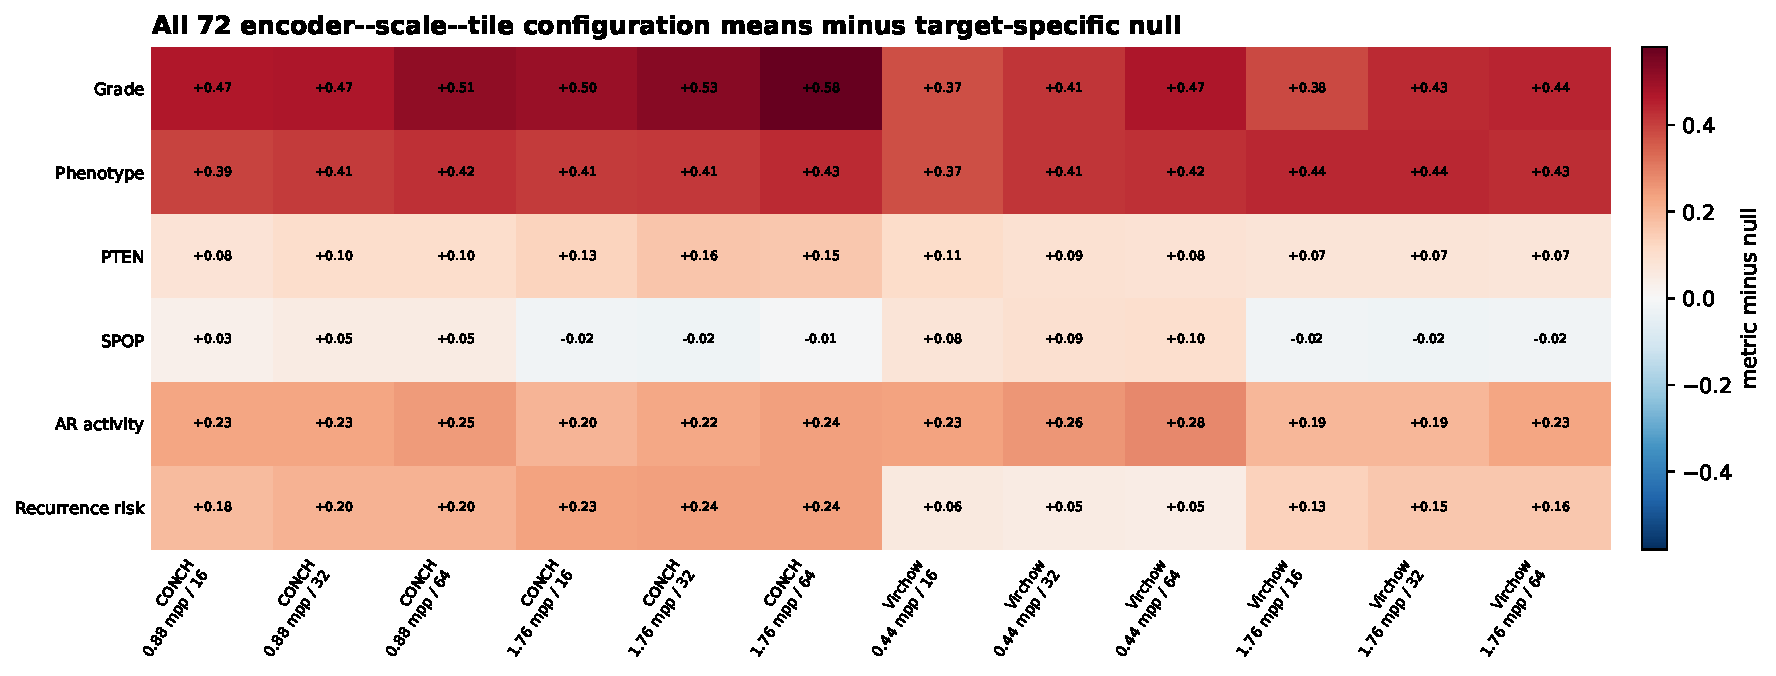
\includegraphics[width=\textwidth]{figures/sfig1_full_stability_grid.pdf}
\caption{\textbf{Complete encoder--scale--tile configuration grid.} Each cell is the mean
of five sampling seeds minus the target-specific metric null. Columns retain encoder,
physical scale, and tile budget; rows retain target identity. Values reuse cohorts and folds
and therefore describe correlated setting sensitivity rather than independent validation.}
\label{fig:supp-full-grid}
\end{figure}

\begin{table}[H]
\centering
\scriptsize
\caption{Observed ranges across 12 correlated encoder--scale--tile configurations. Mean and range summarize the five-seed configuration values; null-straddling is the number of configurations whose observed seed range crossed the target-specific null, out of 12. These are sensitivity summaries, not independent validations.}
\label{tab:supp-stability}
\begin{tabular}{@{}p{0.10\textwidth}p{0.19\textwidth}p{0.08\textwidth}p{0.10\textwidth}p{0.23\textwidth}p{0.15\textwidth}@{}}
\toprule
Target & Metric & Null & Mean & Range & Null-straddling \\
\midrule
Grade & Patient Spearman rho & 0.0 & 0.464 & 0.271 to 0.646 & 0/12 \\
Phenotype & Patient AUROC & 0.5 & 0.915 & 0.845 to 0.965 & 0/12 \\
PTEN & Patient AUROC & 0.5 & 0.602 & 0.519 to 0.717 & 0/12 \\
SPOP & Patient AUROC & 0.5 & 0.523 & 0.348 to 0.679 & 8/12 \\
AR activity & Patient Spearman rho & 0.0 & 0.230 & 0.136 to 0.297 & 0/12 \\
Recurrence risk & Patient C-index & 0.5 & 0.657 & 0.481 to 0.755 & 1/12 \\
\bottomrule
\end{tabular}
\end{table}


The full contrast-level source contains 390 seed-matched comparisons. To expose their
direction and spread without treating them as independent observations,
Supplementary Table~\ref{tab:supp-contrast-summary} summarizes every target within each registered contrast
family. Median and range describe technical sensitivity; null-crossing counts describe a
change in the target-specific chance relation, not a population-level hypothesis test.

\begin{table}[H]
\centering
\scriptsize
\caption{Complete summary of the 390 seed-matched setting contrasts. Delta direction is setting B minus setting A in the named contrast.}
\label{tab:supp-contrast-summary}
\begin{tabular}{@{}p{0.15\textwidth}p{0.11\textwidth}p{0.06\textwidth}p{0.10\textwidth}p{0.17\textwidth}p{0.10\textwidth}p{0.08\textwidth}@{}}
\toprule
Contrast & Target & Pairs & Median delta & Range & Null crossing & Exact ties \\
\midrule
Shared 1.76 mpp - native scale & Grade & 30 & +0.032 & -0.081 to +0.161 & 0 & 0 \\
Shared 1.76 mpp - native scale & Phenotype & 30 & +0.029 & -0.075 to +0.102 & 0 & 0 \\
Shared 1.76 mpp - native scale & PTEN & 30 & +0.026 & -0.108 to +0.154 & 0 & 0 \\
Shared 1.76 mpp - native scale & SPOP & 30 & -0.091 & -0.235 to +0.046 & 19 & 0 \\
Shared 1.76 mpp - native scale & AR activity & 30 & -0.039 & -0.083 to +0.033 & 0 & 0 \\
Shared 1.76 mpp - native scale & Recurrence risk & 30 & +0.056 & +0.015 to +0.188 & 1 & 0 \\
Virchow - CONCH at 1.76 mpp & Grade & 15 & -0.105 & -0.228 to -0.049 & 0 & 0 \\
Virchow - CONCH at 1.76 mpp & Phenotype & 15 & +0.008 & -0.043 to +0.083 & 0 & 1 \\
Virchow - CONCH at 1.76 mpp & PTEN & 15 & -0.081 & -0.162 to -0.003 & 0 & 0 \\
Virchow - CONCH at 1.76 mpp & SPOP & 15 & +0.012 & -0.104 to +0.101 & 4 & 0 \\
Virchow - CONCH at 1.76 mpp & AR activity & 15 & -0.022 & -0.066 to +0.060 & 0 & 0 \\
Virchow - CONCH at 1.76 mpp & Recurrence risk & 15 & -0.085 & -0.125 to -0.057 & 0 & 0 \\
64 tiles - 16 tiles & Grade & 20 & +0.061 & -0.054 to +0.265 & 0 & 0 \\
64 tiles - 16 tiles & Phenotype & 20 & +0.028 & -0.037 to +0.075 & 0 & 1 \\
64 tiles - 16 tiles & PTEN & 20 & +0.003 & -0.079 to +0.079 & 0 & 0 \\
64 tiles - 16 tiles & SPOP & 20 & +0.026 & -0.114 to +0.084 & 5 & 0 \\
64 tiles - 16 tiles & AR activity & 20 & +0.034 & -0.064 to +0.146 & 0 & 0 \\
64 tiles - 16 tiles & Recurrence risk & 20 & +0.017 & -0.060 to +0.041 & 0 & 0 \\
\bottomrule
\end{tabular}
\end{table}


Supplementary Figure~\ref{fig:supp-setting-contrasts} visualizes the same paired contrasts and preserves their direction:
shared scale minus native scale, Virchow minus CONCH at the shared scale, and 64 minus 16
tiles. A positive value therefore has meaning only within the named comparison.

\begin{figure}[H]
\centering
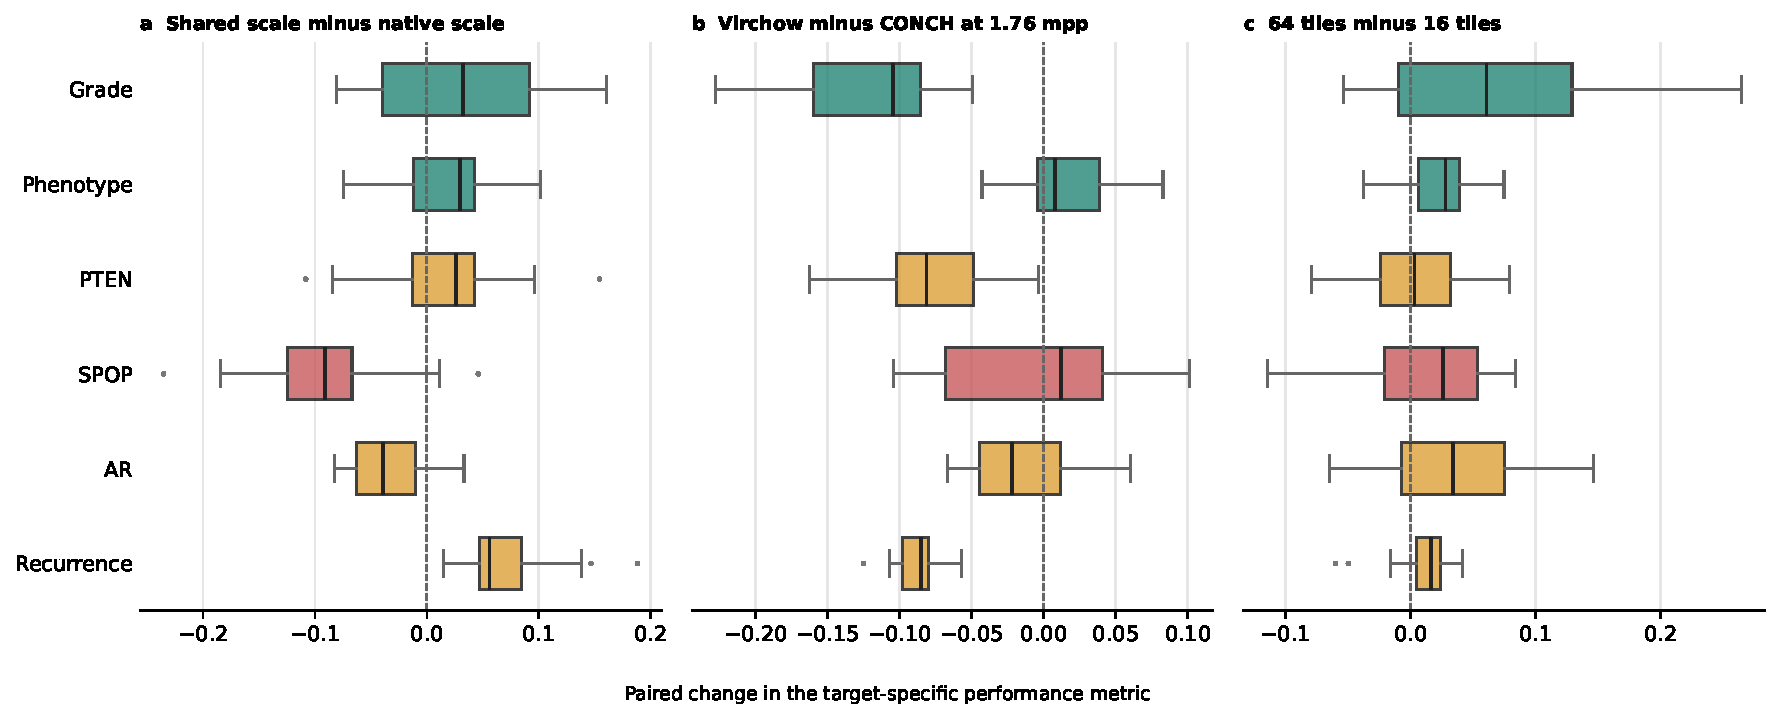
\includegraphics[width=\textwidth]{figures/fig5_setting_contrasts.pdf}
\caption{\textbf{Seed-matched encoder, physical-scale, and tile-budget contrasts.}
Each box summarizes paired performance changes for one target while preserving the sampling
seed. \textbf{a}, Shared physical scale minus encoder-native scale. \textbf{b}, Virchow minus
CONCH at the shared 1.76-micrometre-per-pixel scale. \textbf{c}, 64 minus 16 tiles per slide.
All comparisons reuse cohorts and folds and do not define a universally preferable setting.}
\label{fig:supp-setting-contrasts}
\end{figure}


\section*{S9. Endpoint hierarchy and paired outcome increments}

Reconstructed with-tumor recurrence, strict recurrence-only, TCGA-CDR PFS, TCGA-CDR DFS,
and official PFI retained separate identifiers. On the 270-patient target frame,
reconstructed recurrence had 57 events and official PFI had 42. Paired increment analyses
used 153 complete cases, with 30 and 15 events respectively. All official-PFI paired
C-index and IBS intervals included zero.

Supplementary Table~\ref{tab:supp-endpoints} defines the endpoint IDs, their roles, metrics, and the
non-equivalence boundary that prevents a result under one recurrence definition from being
silently relabeled as another.

The transferred image-risk score was fitted with a Cox model in LEOPARD and applied to
TCGA-PRAD without target-cohort refitting. Its principal-component dimension sweep was
exploratory and was not nested inside an outer evaluation. Paired TCGA comparisons used the
same complete-case patients and bootstrap draw for the reference and augmented models.
C-index improvement was augmented minus reference; integrated Brier score improvement was
reference minus augmented, so positive values favored augmentation under both definitions.
The Cox model estimates relative event hazard under censoring, while integrated Brier score
summarizes time-dependent prediction error and is lower when predictions are better.

The comparison names in Supplementary Tables~\ref{tab:supp-outcome-reconstructed} and
\ref{tab:supp-outcome-official-pfi} have the following meaning. ``Grade + image vs grade''
and ``full clinical + image vs full clinical'' test augmentation by the transferred image
risk score; here the full clinical reference contains grade, age, PSA, pathological T stage,
and surgical-margin status. ``Image vs grade'' and ``image vs full clinical'' compare
non-nested reference choices rather than incremental models. In the separate prespecified
hierarchy, M4 contains grade, PSA, pathological T stage, surgical-margin status, and
tissue-source site, whereas M5 adds the image risk score. Thus ``full clinical + site + image
vs full clinical + site'' is the M5--M4 comparison. These labels describe model contents,
not evidence that the image score adds clinical value.

\begin{table}[H]
\centering
\scriptsize
\caption{Registered endpoint hierarchy and non-equivalence boundaries. Primary rows define known-target recoverability, secondary rows test conditional or horizon-specific questions, and exploratory rows audit recurrence definitions. Each row keeps its own metric and boundary; endpoint IDs are not interchangeable outcomes.}
\label{tab:supp-endpoints}
\begin{tabular}{@{}p{0.05\textwidth}p{0.12\textwidth}p{0.16\textwidth}p{0.14\textwidth}p{0.15\textwidth}p{0.17\textwidth}@{}}
\toprule
ID & Hierarchy & Target or endpoint & Metric & Role & Boundary \\
\midrule
E01 & Primary & Continuous or ordinal marker target & Spearman rho & Known-target recoverability & Not a disease decision \\
E02 & Primary & Binary marker target & AUROC & Known-target recoverability & Not a molecular diagnosis \\
E03 & Secondary & PTEN or AR beyond grade & Delta AUROC or delta R2 & Conditional uniqueness beyond grade & Not evidence of functional use \\
E04 & Exploratory & Reconstructed recurrence with tumor & C-index, time-dependent AUROC, and IBS & Recurrence alignment & Not official PFI \\
E05 & Exploratory & Strict recurrence only & C-index and time-dependent AUROC & Sensitivity analysis & Not official PFI \\
E06 & Exploratory & TCGA-CDR PFS & C-index, time-dependent AUROC, and landmark AUROC & Sensitivity analysis & Not relabeled as PFI \\
E07 & Exploratory & TCGA-CDR DFS & C-index, time-dependent AUROC, and landmark AUROC & Sensitivity analysis & Not relabeled as PFI \\
E08 & Exploratory & Official TCGA-CDR PFI & C-index and endpoint concordance & Outcome alignment & Not equivalent to reconstructed recurrence \\
E09 & Secondary & Three- and five-year landmarks & Landmark C-index or AUROC & Sensitivity analysis & Not equivalent to a time-to-event analysis \\
\bottomrule
\end{tabular}
\end{table}



Supplementary Tables~\ref{tab:supp-outcome-reconstructed} and
\ref{tab:supp-outcome-official-pfi} retain the full frozen-risk and paired comparison frames.
The paired rows use identical patients and bootstrap draws within an endpoint. The two
endpoint tables must not be pooled because their event definitions and event counts differ.

\begin{table}[H]
\centering
\scriptsize
\caption{Complete frozen-risk and paired comparisons for the reconstructed recurrence-with-tumor endpoint. Paired rows use the same patients and bootstrap draws. C-index delta is augmented or first model minus reference; IBS delta is reference minus augmented or first model, so positive values favor the augmented or first model. Intervals are 95 percent patient-bootstrap intervals; accounting reports undefined draws out of 2,000.}
\label{tab:supp-outcome-reconstructed}
\begin{tabular}{@{}p{0.23\textwidth}p{0.11\textwidth}p{0.04\textwidth}p{0.06\textwidth}p{0.08\textwidth}p{0.16\textwidth}p{0.11\textwidth}@{}}
\toprule
Comparison & Metric & n & Events & Estimate & Interval & Undefined / 2,000 \\
\midrule
Frozen image-risk score & C-index & 270 & 57 & +0.673 & +0.587 to +0.759 & 0/2,000 \\
Full clinical + image vs full clinical & C-index & 153 & 30 & -0.001 & -0.020 to +0.019 & 0/2,000 \\
Full clinical + image vs full clinical & IBS (0.5--5 years) & 153 & 30 & +0.004 & -0.003 to +0.011 & 0/2,000 \\
Grade + image vs grade & C-index & 153 & 30 & +0.083 & +0.012 to +0.157 & 0/2,000 \\
Grade + image vs grade & IBS (0.5--5 years) & 153 & 30 & +0.005 & -0.002 to +0.013 & 0/2,000 \\
Image vs full clinical & C-index & 153 & 30 & -0.173 & -0.312 to -0.053 & 0/2,000 \\
Image vs full clinical & IBS (0.5--5 years) & 153 & 30 & -0.017 & -0.044 to +0.011 & 0/2,000 \\
Image vs grade & C-index & 153 & 30 & +0.025 & -0.137 to +0.176 & 0/2,000 \\
Image vs grade & IBS (0.5--5 years) & 153 & 30 & -0.001 & -0.019 to +0.017 & 0/2,000 \\
Add image to clinical + site (M5 vs M4) & C-index & 153 & 30 & -0.006 & -0.021 to +0.006 & 0/2,000 \\
Add image to clinical + site (M5 vs M4) & IBS (0.5--5 years) & 153 & 30 & +0.001 & -0.003 to +0.005 & 0/2,000 \\
\bottomrule
\end{tabular}
\end{table}



\begin{table}[H]
\centering
\scriptsize
\caption{Complete frozen-risk and paired comparisons for official TCGA-CDR PFI. Paired rows use the same patients and bootstrap draws. C-index delta is augmented or first model minus reference; IBS delta is reference minus augmented or first model, so positive values favor the augmented or first model. Intervals are 95 percent patient-bootstrap intervals; accounting reports undefined draws out of 2,000.}
\label{tab:supp-outcome-official-pfi}
\begin{tabular}{@{}p{0.23\textwidth}p{0.11\textwidth}p{0.04\textwidth}p{0.06\textwidth}p{0.08\textwidth}p{0.16\textwidth}p{0.11\textwidth}@{}}
\toprule
Comparison & Metric & n & Events & Estimate & Interval & Undefined / 2,000 \\
\midrule
Frozen image-risk score & C-index & 270 & 42 & +0.586 & +0.482 to +0.689 & 0/2,000 \\
Full clinical + image vs full clinical & C-index & 153 & 15 & +0.030 & -0.003 to +0.073 & 0/2,000 \\
Full clinical + image vs full clinical & IBS (0.5--5 years) & 153 & 15 & +0.004 & -0.002 to +0.013 & 0/2,000 \\
Grade + image vs grade & C-index & 153 & 15 & +0.032 & -0.040 to +0.126 & 0/2,000 \\
Grade + image vs grade & IBS (0.5--5 years) & 153 & 15 & +0.001 & -0.002 to +0.004 & 0/2,000 \\
Image vs full clinical & C-index & 153 & 15 & -0.134 & -0.365 to +0.084 & 0/2,000 \\
Image vs full clinical & IBS (0.5--5 years) & 153 & 15 & -0.001 & -0.017 to +0.017 & 0/2,000 \\
Image vs grade & C-index & 153 & 15 & -0.163 & -0.403 to +0.069 & 0/2,000 \\
Image vs grade & IBS (0.5--5 years) & 153 & 15 & -0.009 & -0.024 to +0.005 & 0/2,000 \\
Add image to clinical + site (M5 vs M4) & C-index & 153 & 15 & -0.004 & -0.016 to +0.006 & 0/2,000 \\
Add image to clinical + site (M5 vs M4) & IBS (0.5--5 years) & 153 & 15 & -0.000 & -0.002 to +0.002 & 0/2,000 \\
\bottomrule
\end{tabular}
\end{table}


Supplementary Figure~\ref{fig:supp-outcome-contrasts} plots the paired intervals from the two
tables on a common positive-favors-first-or-augmented convention; endpoint-specific panels
remain separate because their event definitions and counts differ.

\begin{figure}[H]
\centering
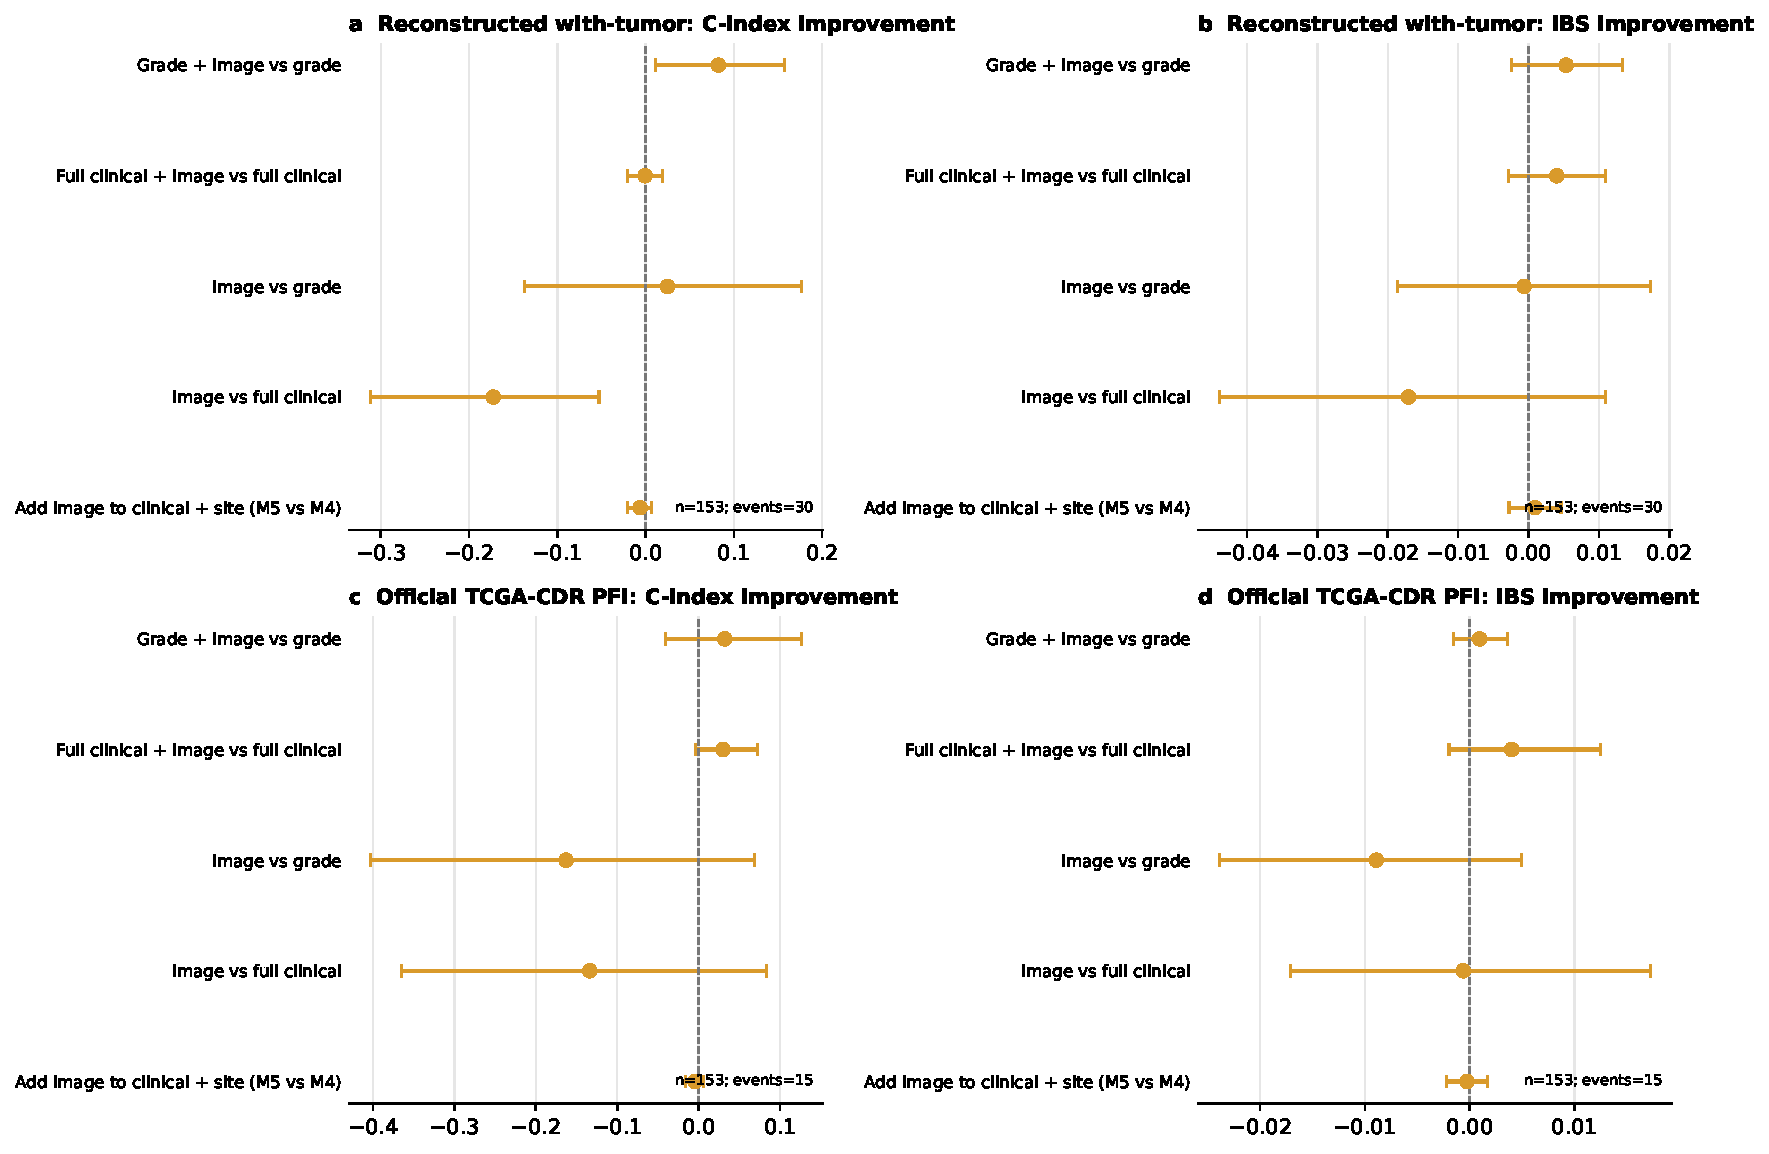
\includegraphics[width=\textwidth]{figures/fig6_outcome_contrasts.pdf}
\caption{\textbf{Complete paired outcome-comparison family across non-equivalent endpoints.}
Rows compare the image score with grade or fuller clinical references, or compare nested
clinical models, on the same patients and bootstrap draws. \textbf{a,b}, Reconstructed
with-tumor C-index and integrated-Brier-score improvements. \textbf{c,d}, Corresponding
official TCGA-CDR PFI comparisons. Positive values favor the first, augmented, or more
complete model under the registered delta definition.}
\label{fig:supp-outcome-contrasts}
\end{figure}


\section*{S10. Multiplicity, undefined draws, and power boundaries}

The saved discovery family contained 17 tests with Benjamini--Hochberg false-discovery-rate
control. External and representation checks of an existing target were qualification
analyses. Missing intervals, missing event counts, single-class sites, and underpowered
endpoint rows remained explicit. No non-significant result was interpreted as biological
absence.

Where saved sources supported it, uncertainty used 95\% percentile patient-bootstrap
intervals. The bootstrap resampled patients with replacement and recomputed the statistic;
AR site analyses instead resampled patients as clusters around a slide-level effect. Paired
survival contrasts used identical draws for both models. Requested, valid, and undefined
replicate counts were reported when retained and otherwise marked unavailable. No missing
or unevaluable outcome was converted to a negative label, and multiple imputation was not
introduced retrospectively.

The promoted derivative evidence retains the family-level multiplicity contract but does not
contain a complete row-level table of all raw and adjusted $p$ values. Those values were not
reconstructed from prose. Supplementary Table~\ref{tab:supp-missingness-summary} instead reports every
retained availability and bootstrap-accounting state across the promoted figure-source
tables, making clear which limitations arise from missing intervals, event counts,
single-class sites, or legacy replicate accounting.

\begin{table}[H]
\centering
\scriptsize
\caption{Row-level availability and uncertainty-accounting states retained in the promoted evidence. Counts are source-table rows, not patients or independent tests; unavailable quantities and undefined single-class estimates were preserved rather than reconstructed.}
\label{tab:supp-missingness-summary}
\begin{tabular}{@{}p{0.27\textwidth}p{0.48\textwidth}p{0.10\textwidth}@{}}
\toprule
Evidence component & Availability/accounting state & Rows \\
\midrule
External transport & Interval not saved & 5 \\
External transport & Replicate accounting not saved & 2 \\
Molecular alignment & Bootstrap accounted & 5 \\
Molecular alignment & Event count not applicable & 2 \\
Molecular alignment & Event count not recorded in source & 4 \\
Molecular alignment & Primary metric undefined & 1 \\
Conditional and site audits & Event count not applicable & 9 \\
Conditional and site audits & Event count not recorded in source & 2 \\
Outcome & Bootstrap accounted & 22 \\
\bottomrule
\end{tabular}
\end{table}



\section*{S11. Claim--evidence and numeric lineage}

Each main claim is connected to a PBV source claim, a target identifier, required evidence
axes, and a functional-use status. Each reported headline number is linked to a source ID,
semantic key, field, and display rule. The full machine-readable records are
\path{provenance/claim_evidence_matrix.csv} and
\path{provenance/numeric_qa_mapping.csv}.

Supplementary Table~\ref{tab:supp-claim-matrix} exposes the manuscript claim ID, source-claim lineage,
registered target IDs, evidence state, and functional-use status together. It is the final
check that a representation-level result has not been promoted to a locked-head or clinical
claim.

\begin{table}[H]
\centering
\scriptsize
\caption{Claim--evidence and functional-use boundary. A identifiers denote this manuscript's claims, C identifiers denote promoted source claims, and T identifiers denote registered targets. The state summarizes the qualified evidence, whereas functional use records whether a locked-head intervention was tested; recoverability alone does not establish head use.}
\label{tab:supp-claim-matrix}
\begin{tabular}{@{}p{0.05\textwidth}p{0.12\textwidth}p{0.16\textwidth}p{0.23\textwidth}p{0.13\textwidth}@{}}
\toprule
Claim & Source claims & Targets & State & Functional use \\
\midrule
A01 & C01; C08 & T01; T02; T03; T04; T05; T06 & Descriptive framework & Not tested \\
A02 & C02 & T01; T02 & Transportable & Not tested \\
A03 & C03 & T03 & Context-sensitive & Not tested \\
A04 & C05 & T05 & Context-sensitive & Not tested \\
A05 & C04 & T04 & Unsupported in frozen design & Not tested \\
A06 & C06; C07 & T06 & Context-sensitive & Not tested \\
A07 & C08 & T01; T02; T03; T04; T05; T06 & Descriptive framework & Not tested \\
A08 & QFM-FM6-SUMMARY; QFM-FM6-CONTRASTS & T01 & Internal exploratory & Internal exploratory only \\
A09 & QFM-FM6-CONTRASTS & T01 & Context-sensitive & Internal exploratory only \\
A10 & none & T01; T02; T03; T04; T05; T06 & Deferred follow-up & Not claimed \\
A11 & QFM-FM6-SITE-HELDOUT; QFM-FM6-LEOPARD-EXTERNAL; QFM-FM6-CHIMERA-EXTERNAL & T01 & encoder specific external transport & external encoder specific whole tissue \\
\bottomrule
\end{tabular}
\end{table}



\section*{S12. Reproducibility and known limitations}

The manuscript builder first verifies every source path against its registered byte count
and SHA-256 hash. It then generates new QFM-owned figures and tables from those sources.
No PBV-generated PDF, PNG, or TeX table is copied. The PBV project remains owner of the
frozen analyses, while QFM owns the derivative alignment narrative.

For the FM6 extension specifically, internal clean-rerun handoff required 20/20 nonvolatile
output hashes, unchanged headline numbers, and unchanged gates. Both encoders retained
R=whole-tissue recoverability, A=internal disease association, and U=exploratory whole-tissue
functional sensitivity. Site-heldout transport was encoder-specific; the locked LEOPARD family
failed or remained inconclusive for both encoders; and Virchow alone passed the CHIMERA external
whole-tissue gate. T therefore passed only at an encoder- and cohort-specific level, while strong
H2 remained prohibited. These gate labels describe evidence scope rather than a sequence of
clinical validation levels.

Unequal availability of external target-matched cohorts limits comparison between target
classes. The correlated grid is not independent validation; site effects are not causal
acquisition effects; and recurrence endpoints are not interchangeable. The grade analysis
includes locked BCR heads and target-erasure experiments, including one encoder-specific
external whole-tissue pass. Its detector did not pass the independent-domain sensitivity gate,
refitted heads could compensate internally, and the limited ISUP-only comparison was not a
sufficient clinical-increment study. The present paper therefore establishes candidate shared
interpretive coordinates and bounded, model-specific grade sensitivity, not complete explanation
of AI decisions. Residual or unknown-feature marker discovery is reserved for a separate study.
